\section[CPU]{Design of a 16 bit Central Processing Unit (CPU)} 
A Central Processing Unit (CPU) is the electronic circuit withing a computer that executes instructions that make up a computer.The CPU, by all means, is one of the most important component of a computer system. Since computers vary from one another by size and complexity, so does there CPUs vary. In fact, the power of a computer is a measure of the efficiency and speed of its processor. CPUs can be found in every computer. From the cheap microcontrollers found in toys to the multi-million dollar, number-crunching Super Computers used in large organizations.  The CPU performs basic arithmetic, logic, input/output and controlling operations as specified by the instruction. The CPU is to a computer what a brain is to a living organism.

The concept of a CPU and a computer as a whole were explained in a course I took in my third year in University. The course (Computational Structures) explained in details how a computer system was designed from scratch. The course explained the design of a computer system from  the designing of an Instruction Set Architecture (ISA) to implementing the design in hardware. The course was taught in a very theoretical way (as expected) and there was a little bit of paucity of depth. This project was undertaken with the hope that this will be remedied.

This is not a super scalar processor. It is written in Hardware Description Language (HDL), flashed unto a Field Programmable Gate Array (FPGA) and tested. This CPU takes multiple instructions to execute the simplest of instructions. It’s aimed at a level to educate myself.

I hope to implement the following.
\begin{enumerate}
\item A 16-bit CPU Modified Harvard Architecture core
\item 16 16-bit general registers.
\item Basic arithmetic operations, shifts, additions.
\item Branching.
\item A control unit to keep everything in lock-step.
\item Synthesized RAM for instruction and data storage.
\item An in-order CPU with no real pipelining as such
\end{enumerate}

\subsection[ISA]{Choice of ISA}
An Instruction Set Architecture (ISA) is a very important feature of a processor. It is an abstract model of a computer. An ISA defines the supported data types, the registers, the hardware support for managing main memory fundamental features and the input/output model of an ISA. The ISA of a processor cannot be changed once created because it basically dictates the hardware implementation of the processor.
ISAs are classified based on architectural complexity into two.
\begin{enumerate}
\item \textbf{Complex Instruction Set Computer (CISC):} This ISA has many specialized instructions, some of which may only be rarely used in practical programs.
\item \textbf{Reduced Instruction Set Computer (RISC):} This ISA has a small set of simple and general instructions, rather than a large set of complex and specialized instructions. It allows a CPU to have fewer cycles per instruction (CPI) than a complex instruction set computer (CISC)(ref).
\end{enumerate}

The design of an Intruction Set Architecture is not an easy feat. For this reason and time constraints, I opted to design the CPU based on a scratch built ISA designed by Colin "Domipheus" Riley called the Test Processing Unit (TPU). It has a intermediate level of complexity and difficulty to  implement. It also gives room for restructuring as the designer is easily accessible for questions and help. The ISR fufils all the requirements stated above and more.

\begin{figure}[p]
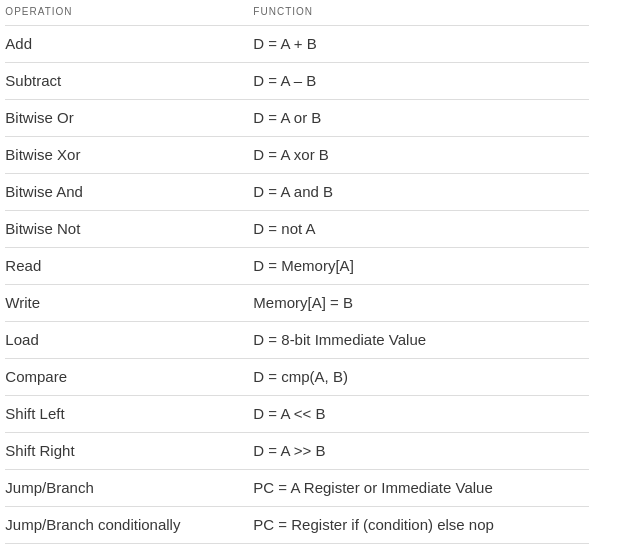
\includegraphics[width=16cm]{Instructions}
\centering
\caption{The Instructions supported by the TPU ISA}
\centering
\label{fig:instr}

\end{figure}


Migen was chosen as the HDL of choice because of its simplicity and Python-like syntax. The ISA supports 14 different instructions. They are the basic and the most found instructions in similar RISC ISAs. The instructions are of three categories 

\begin{enumerate}
\item Arithmetic Instructions : These instructions are basically for basic numeric operations. This include Addition(ADD) and Subtraction(SUB). All other arithmetic instructions such as Division and Multiplication can and would be implemented as a function of some basic instructions
\item Logical Instructions : These instructions are basically for basic Logical operations. They are carried out both on numerical data and logical data. 
\item Conditional and Branching Instructions
\item Memory accessing Instructions:These instructions are very important in the storage and retrieval of data in the memory of a system. They include SAVE, LOAD and WRITE instructions.
\end{enumerate}

There is a need to define the structure of instructions for the ISA. It is a common thing to put the OPCODE first before the ARGUEMENTS of the particular command. An intruction can have a number of arguments or inputs depending on it structure. There are quite a number of ways by which instructions are structured in this regard. This is shown in the Figure \ref{fig:instr}. Some instruction take, as arguements, the regidters number. This means that the operation is performed on the content of the registers and stored in a particular output register. Some other instruction takes the constant inside the instruction and directly perform operation on them. All these depend on the kind of operation to be carried out on the data. 
An instruction is basically a 16-bit nuumber and it contains both the operation and the operands(Register number or constant). The OPCODE is 4-bit wide and is enough for our 14 operations with space left for two more in the future. The OPCODE starts from the 15th bit and ends on the 12th bit. This is consistent across all instructions . The other forms of instruction bit assignment are shown in Figure \ref{fig:inst_bit_srt}. 

\begin{figure}[p]

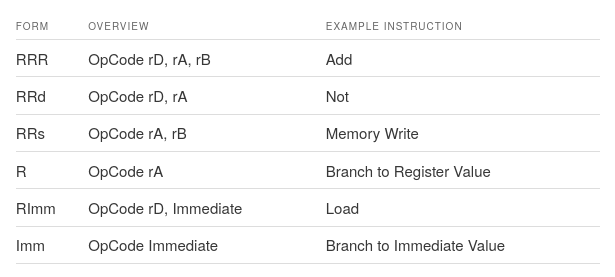
\includegraphics[width=16cm]{opcode_Structure}
\centering
\caption{Instructions Structure.}
\centering
\label{fig:inst_str}
\end{figure}


\begin{figure}[p]

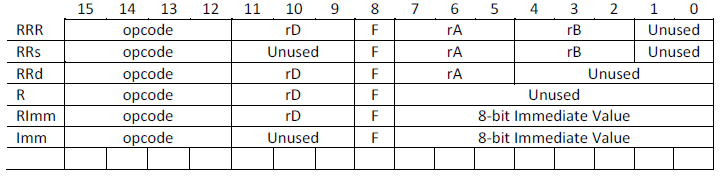
\includegraphics[width=15cm]{forms_bits_organization}
\centering
\caption{Instructions bit Assignments.}
\centering
\label{fig:inst_bit_srt}
\end{figure}

A very important thing to note at this point is the fact that the load value is unable to load into a register a 16-bit value at once. This is because the instruction itself is 16 bit and still has to contain other things like the OPCODE and other parameters just as important as the data. This is remedied by allowing the processor to load into the upper and lower part of a register independently. Thsi is controlled by the bit number eight. This parameter is found in all instructions but used only by very few ones.

It is also important to know that our registers are demoted by three bits of the instruction. This allows for referencing only eight registers. This is a core and intrinsic part of the ISA and cannot be changed wwithout changing the ISA itself.
The processor does not possess a special register for special numbers and special functions such as the Stack pointer in the Beta machine. This greatly simplifies the complexity of the system at the expense of its performance.  

\subsection{Designing the Register File}
The Register File is a part of the processor that contains the registers. There are eight 16-bit individual registers that make up the Register File. The Register File is the storage medium for the processor. It is where data is stored during operation. They are usually made of the fastest kind of memory element to reduce access time during operation. 

The Register Files takes in one 16-bit data inputs and two 16-bit data outputs. These outputs allow data from two different register to be available at the output buses for the ALU. The choice of register is made by the output bus select inputs. These inputs are three bits and are just enough to adderess the eight registers of the register files. The destination of the data on the input bus is also controlled by a write enable bit and a three bit select input. Therefore, data can be written to the Register files when it is needed. Finally, there is a clock input and an enable bit to activate the whole Register file as a whole.

During the implementation of this module, I wrote the program in such a way that the output from the Register File is held until the select pin changes the choice of register. In other words, if the Register File is enabled , it will always output the content of two registers based on their respective select input. I wrote a testbench to simulate every possible scenarios and I was able to make the Register File perform as follows.

\begin{figure}[p]

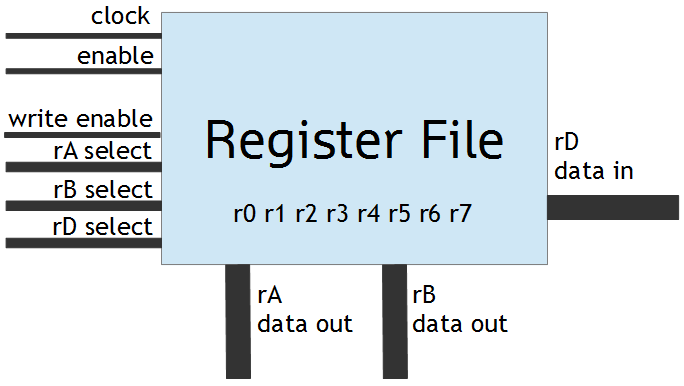
\includegraphics[width=12cm]{reg_file}
\centering
\caption{Diagramatic representation of an Register File}
\centering
\label{fig:decoder}
\end{figure}







\subsection{Designing the Instruction Decoder}
The decoder is a very important section of a microprocessor. it is responsible for extracting necessary data and commands from an instruction. In other words, it is responsible for pulling bits out from the instruction stream and sending them on to the other units we connect to: The Register file, ALU, and Control unit(s).

The Instruction decoder require the fillowing inputs.
\begin{itemize}
\item Clock input
\item An enable input
\item Instruction input
\end{itemize} 

The outputs include the following 
\begin{itemize}
\item the Alu OPCODE.
\item Selection lines for the Register file (rD, rA and rB).
\item Write enable to enable writing into the Register file.
\item The Immediate(Constant) value from the instruction.
\end{itemize}

The ALU OPCODE also contains the flag. The flag signifies different things for different commands. The instructions that require the flag bit make use of it in the code and others that don't simply discard and ignore its existence. For the case of memory based commands like LOAD and WRITE, it is for putting the immediate value in the upper or lower eight bit part of the selected register rD. For that of JUMP, it is for signaling if the processor should jump to the immediate value or to the value stored in the given register. Figure  \ref{fig:opcode_bit_flag} shows the list of the commands, their OPCODES, and the status of the write enable and flag. Figure \ref{fig:decode} shows a diagrametric representation of an Instruction decoder.



\begin{figure}[p]

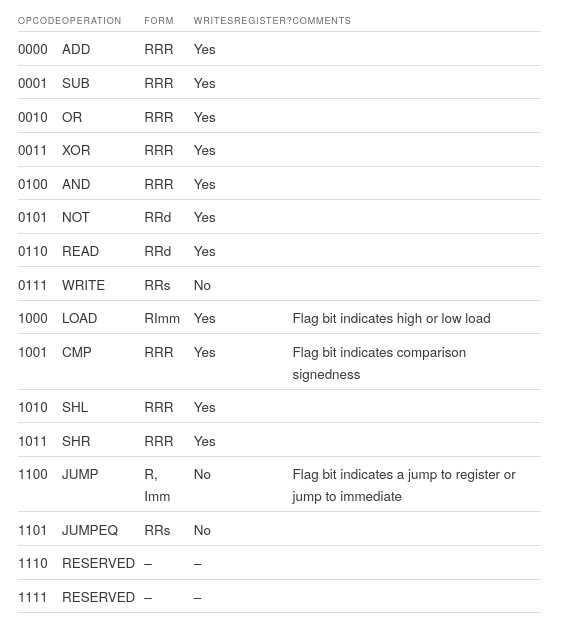
\includegraphics[width=13cm]{opcode_with_flag}
\centering
\caption{OPCODES and Instruction Structure.}
\centering
\label{fig:opcode_bit_flag}
\end{figure}


\begin{figure}[p]

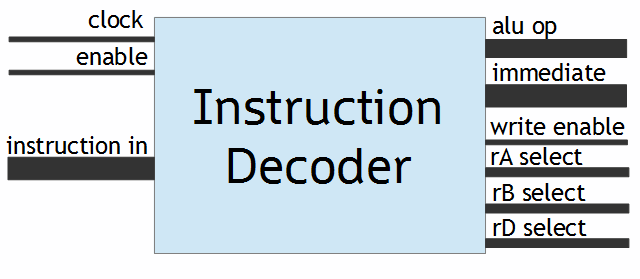
\includegraphics[width=12cm]{decoder}
\centering
\caption{Diagramatic representation of an Instruction Decoder}
\centering
\label{fig:decode}
\end{figure}



\subsection{Designing the Arithmetic and Logical Unit}

In TPU, we are only doing single cycle operations. Whilst a whole instruction will take multiple cycles to complete, the ALU itself will output a result in a single clock cycle. The other cycles are due to decoding, fetching and any writebacks of results which are required. The ALU takes in two 16-bit data input, an ALU opcode and produces the output of the operation after a number of clock cycles. 
Other inputs include clock, enable bit, write-enable bit, 16-bit program counter and eight bit immediate value. The program counter and the immediate value inputs are for storing important data required for loading data into the register file. in the case of the program counter, the important data is the next address to go to. This is an important reason for outputing a shouldBranch output bit. This helps to signify when a jump is required during the execution of a particular instruction.

Our ALU process which runs on a rising clock edge, when enable bit is active, will immediately enter a case statement dependent on the alu operation forwarded from the decoder and inputed though the ALUop input. 
Each if block within the case statement will write to elements of an internal register sresult, which is 18 bits wide, to accommodate carry or overflow status. There is also an internal signal for the shouldBranch output.The shouldBranch output is not computed but inferred from the opcode. This is because of the fact that we already know the number of instructions that requires branching. 
The ALU code was written to be as optimized as possible as it - just as others - can cause a serious bottleneck in the operation of the microprocessor.
\begin{figure}[p]
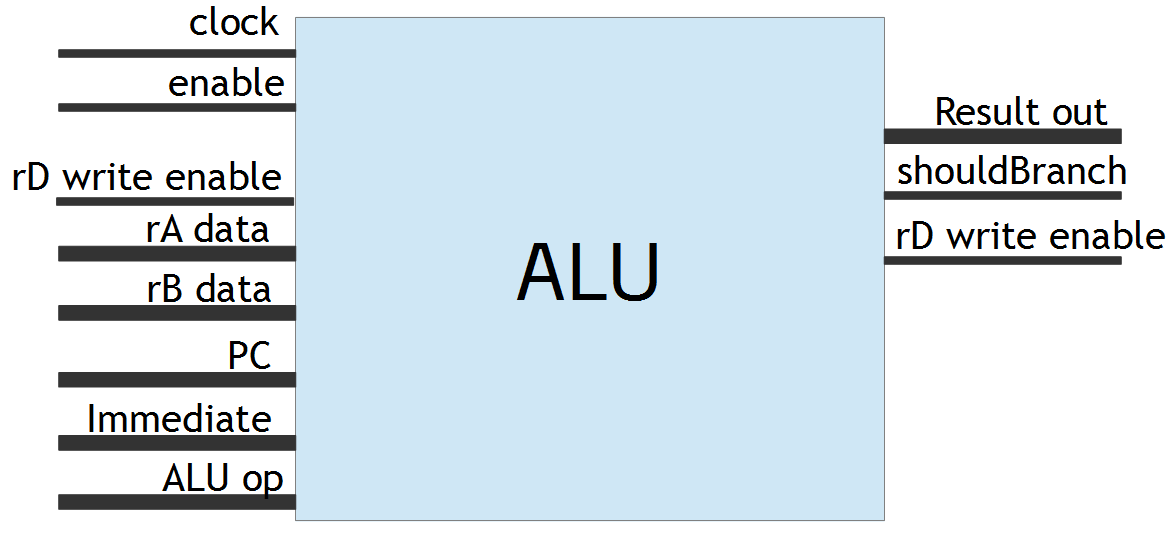
\includegraphics[width=12cm]{alu}
\centering
\caption{Diagramatic representation of the Arithmetic and Logical Unit.}
\centering
\label{fig:alu}
\end{figure}



\subsection{Designing the Control Unit}
During the implementation of the other modules, you will notice the presence of enable bits in all of the modules. This gives us the ability to switch our modules inputs on at will. Each module has a register at its output and it will preserve the output until the enable bit is asserted and the computation is carried out.  
The control unit basically controls the enable bit of every module of the micro processor. it helps in the crude pipelining of data in the processor. 
The control unit is technically a state machine, but for now it’s simple enough we can just classify it as a counter. It is a simple six bit counter. The code was written to shift a bit right through its output and activate the neccessary module. It activates the RAM first since it is where the instruction is fetched and sent to the decoder.


\subsection{Designing the Program Counter}
The Program Counter (PC) is a very important part of a microprocessor. It contains the address (location) of the instruction being executed at the current time.  It helps to simplify the process of jumping and branching to any instruction by allowing this to be done by changing its value.
In the TPU, our PC unit will obviously hold the current PC address, and on command increment it. It has an input for setting the next PC value, and also the ability to stop – stay at the same location – which we need due to our pipeline being several cycles long.

Our PC is basically required to perform one of the following things at a particular time.
\begin{enumerate}
\item Increment PC
\item Set PC to new value
\item Do nothing (halt)
\item Set PC to our reset vector, which is 0x0000.
\end{enumerate}

This means that two bit is enough to tell the PC what to do. This input is the PCin input. The normal state of the PC is when PCin is equal to 0. At this point, the PC simply increments its current value by one as it is the normal feature of programs to execute from top to bottom.

\begin{figure}[p]
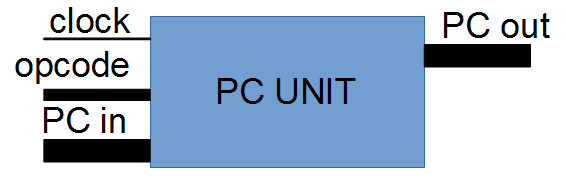
\includegraphics[width=12cm]{pcunit}
\centering
\caption{Diagramatic representation of the Program counter.}
\centering
\label{fig:pcunit}
\end{figure}

\subsection{Testing of Different Modules}
During the process of implementing the ISA in migen, modularity was paramount. This led to the independent development of individual modules albiet the fact that they were designed to work together. The pipeline was established and data is meant to progress or move from the program counter to the RAM to the decoder to the register file to the ALU and back to the register file. This flow is controlled by the control unit. 
The individual modules were tested independently and then chained together for a joint test. The testing takes the form of subjecting each module to certain scenarios and checking and confirming that they react and respond in the appropriate ways. The test cases are written in form of testbenchs. The testbenches are written in python and thus inherits the flexibility of python. This is only hindered by the limitation of FHDL itself.

The first module to be tested was the register file. The module was subjected to the following test:
\begin{enumerate}
\item A constant clock input was fed into the module
\item The enable pin was asserted and numbers were stored in different momory location sequentially
\item The numbers were read out of the memory location and compared to the initial stored ones
\item The enable pin deasserted and random numbers were fed into the input in different memory location.
\item The numbers were read out of the memory location and compared to the initial stored ones.
\item Data was stored and retrieved form the register file at the same time in one clock cycle.

\end{enumerate}
At the end of the testing, all scenarios were handled well and the module performed all operation in one clock cycle as intended


\section{Building of a LoRa Communication Pipe Device} 



\section{Design of a Gas Monitoring Device} 



\section{PCB Making} 

\section{Building of a LoRa Data Concetration Device}

I wrote a testbench to test for different senarios of inputs which are essentially 16 bit integers. I generated a VCD file and displayed the result of the test. This is shown in Figure \ref{fig:Decode_sim}.

\begin{sidewaysfigure}[p]
    \centering
    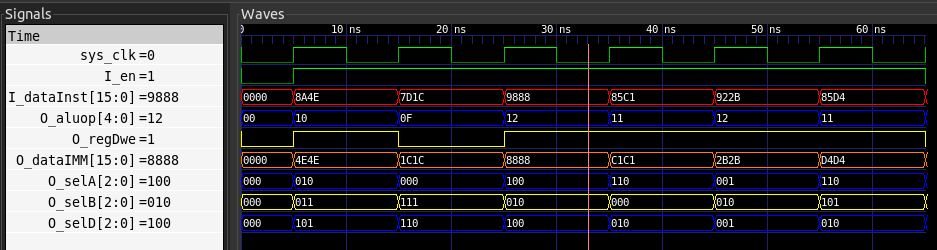
\includegraphics[width=24cm, height=8cm]{Decode_sim}
	\caption{Simulation Diagram for an Instruction Decoder.}
    \label{fig:sim_decode}
\end{sidewaysfigure}

As shown in the  Figure \ref{fig:sim_decode}, the Instruction decoder successfully split the instruction into its various components in a single clock cycle. This is because the system is more of a combinational system with a register at the output.




\begin{figure}[p]
    \centering
    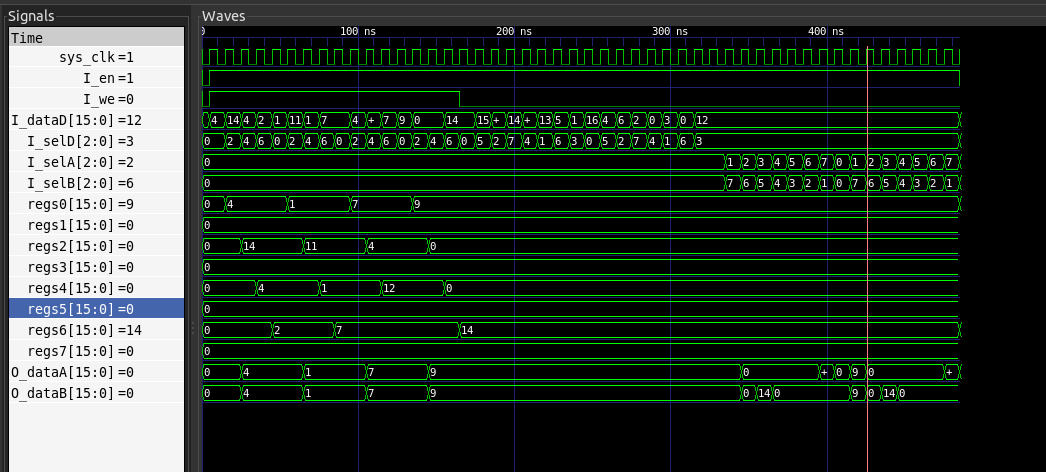
\includegraphics[scale = 0.7]{Reg_file_simulation}
	\caption{Simulation Diagram for an Register FIle.}
    \label{fig:reg_sim}
\end{figure}

\begin{itemize}
\item On each clock cycle and if enabled, update the source A and B register outputs given the selection inputs for A and B
\item On each clock cycle and if enabled, and if the write enable is active, set the internal value of the register D selected to that passed into the selected register value.
\item Fetch data and Write to the same register on the same clock cycles.
\item All operation require only a clock cycle.
\end{itemize} 
